\documentclass[spanish,a4paper,14pt,oneside]{extreport}
 
  %%%%%%%%%%%%%%%%%%%%%%%%%%%%%%%%%%%%%%%%%%%%%%%%%%%%%%%%%%%%%%%%%%%%%%%%%%%%%%%
  \usepackage[dvips]{graphicx}
  \usepackage[dvips]{epsfig}
  \usepackage[utf8]{inputenc}
  \usepackage[spanish]{babel}
  \usepackage{alltt}
  \usepackage{algorithm}
  \usepackage{algorithmic}
  \usepackage{multirow}
  \usepackage[top=2cm, bottom=2cm, left=2cm, right=2cm]{geometry}
   
  %%%%%%%%%%%%%%%%%%%%%%%%%%%%%%%%%%%%%%%%%%%%%%%%%%%%%%%%%%%%%%%%%%%%%%%%%%%%%%%
  \usepackage{array}
  \widowpenalty=5000
  \usepackage{tocloft}
  \renewcommand{\cftchapafterpnum}{\vspace{10pt}}
  \usepackage{eurosym}
  %%%%%%%%%%%%%%%%%%%%%%%%%%%%%%%%%%%%%%%%%%%%%%%%%%%%%%%%%%%%%%%%%%%%%%%%%%%%%%%
   
  \newcommand{\SONY}{{\sc Sony}}
  \newcommand{\MICROSOFT}{{\sc Microsoft}}
  \newcommand{\GCC}{\textsf{\textsc{G}CC}}
  \newcommand{\INTEL}{\textsf{\textsc{I}ntel}}
   
  %%% Traducimos el pseudocodigo
  \renewcommand{\algorithmicwhile}{\textbf{mientras}}
  \renewcommand{\algorithmicend}{\textbf{fin}}
  \renewcommand{\algorithmicdo}{\textbf{hacer}}
  \renewcommand{\algorithmicif}{\textbf{si}}
  \renewcommand{\algorithmicthen}{\textbf{entonces}}
  \renewcommand{\algorithmicrepeat}{\textbf{repetir}}
  \renewcommand{\algorithmicuntil}{\textbf{hasta que}}
  \renewcommand{\algorithmicelse}{\textbf{en otro caso}}
  \renewcommand{\algorithmicfor}{\textbf{para}}
   
  %\newcommand{\RETURN}{\textbf{retornar} }
  \newcommand{\RET}{\STATE \textbf{retornar} }
  \newcommand{\TO}{\textbf{hasta} }
  \newcommand{\AND}{\textbf{y} }
  \newcommand{\OR}{\textbf{o} }
   
  %%%%%%%%%%%%%%%%% Creamos un entorno para listar código fuente %%%%%%%%%%%%%%%
  \newenvironment{sourcecode}
  {\begin{list}{}{\setlength{\leftmargin}{1em}}\item\scriptsize\bfseries}
  {\end{list}}
   
  \newenvironment{littlesourcecode}
  {\begin{list}{}{\setlength{\leftmargin}{1em}}\item\tiny\bfseries}
  {\end{list}}
   
  \newenvironment{summary}
  {\par\noindent\begin{center}\textbf{Abstract}\end{center}\begin{itshape}\par\noindent}
  {\end{itshape}}
   
  \newenvironment{keywords}
  {\begin{list}{}{\setlength{\leftmargin}{1em}}\item[\hskip\labelsep \bfseries Keywords:]}
  {\end{list}}
   
  \newenvironment{palabrasClave}
  {\begin{list}{}{\setlength{\leftmargin}{1em}}\item[\hskip\labelsep \bfseries Palabras clave:]}
  {\end{list}}
   
   
  %%%%%%%%%%%%%%%%%%%%%%%%%%%%%%%%%%%%%%%%%%%%%%%%%%%%%%%%%%%%%%%%%%%%%%%%%%%%%%%
  % Format
  %%%%%%%%%%%%%%%%%%%%%%%%%%%%%%%%%%%%%%%%%%%%%%%%%%%%%%%%%%%%%%%%%%%%%%%%%%%%%%%
  %\usepackage{showframe}
  %\marginparwidth 0mm
  %%\topmargin -4 mm
  %\topmargin -21 mm
  %\headheight 10 mm
  %\headsep 10 mm
   
  %\textheight 229 mm
  %\textheight 246 mm
   
  %\oddsidemargin -5.4 mm
  %\evensidemargin -5.4 mm
  %\oddsidemargin 5 mm
  %\evensidemargin 5 mm
   
  %\oddsidemargin -3 mm
  %\evensidemargin -3 mm
   
  %\textwidth 17 cm
  %\textwidth 15 cm
  %\columnsep 10 mm
   
  \input{amssym.def}
   
  %%%%%%%%%%%%%%%%%%%%%%%%%%%%%%%%%%%%%%%%%%%%%%%%%%%%%%%%%%%%%%%%%%%%%%%%%%%%%%%
   
  \begin{document}
   
  %%%%%%%%%%%%%%%%%%%%%%%%%%%%%%%%%%%%%%%%%%%%%%%%%%%%%%%%%%%%%%%%%%%%%%%%%%%%%%%
  % First Page
  %%%%%%%%%%%%%%%%%%%%%%%%%%%%%%%%%%%%%%%%%%%%%%%%%%%%%%%%%%%%%%%%%%%%%%%%%%%%%%%
   
  \pagestyle{empty}
  \thispagestyle{empty}
   
   
  \newcommand{\HRule}{\rule{\linewidth}{1mm}}
  \setlength{\parindent}{0mm}
  \setlength{\parskip}{2.5mm}
   
  \vspace*{\stretch{0.5}}
   
  \begin{center}
  
\includegraphics[scale=0.8]{images/logo_nuevo}\\[10mm]
  {\Huge Trabajo de Fin de Grado}\\
  \bigskip
  {\LARGE Grado en Ingeniería Informática}\\
  \end{center}
   
  \HRule
  \begin{flushright}
         {\Huge Análisis de los resultados de los sistemas de entrenamiento del Pensamiento Computacional} \\[2.5mm]
         {\Large \textit{Analysis of the results of Computational Thinking training systems}} \\[5mm]
         {\Large Samuel Valcárcel Arce} \\[5mm]
  \end{flushright}
  \HRule
  \vspace*{\stretch{2}}
  \begin{center}
   \Large La Laguna, \today
  \end{center}
   
  \setlength{\parindent}{5mm}
   
  %%%%%%%%%%%%%%%%%%%%%%%%%%%%%%%%%%%%%%%%%%%%%%%%%%%%%%%%%%%%%%%%%%%%%%%%%%%%%%%
  % Signature page (add the official stamp)
  %%%%%%%%%%%%%%%%%%%%%%%%%%%%%%%%%%%%%%%%%%%%%%%%%%%%%%%%%%%%%%%%%%%%%%%%%%%%%%%
  \newpage
  %\cleardoublepage
  \thispagestyle{empty}
   
  Dª. {\bf Coromoto Antonia León Hernández}, con N.I.F. 78.605.216-W
  profesora
  Titular de Universidad
  adscrita al Departamento
  de Lenguajes y Sistemas Informáticos
  de la Universidad de La Laguna, como tutora
   
  \bigskip
  D. {\bf Carlos Segura González}, con N.I.F. 78.704.244-S
  profesor
  Titular
  adscrito al Área
  de Ciencias de la Computación
  del Centro de Investigación Matemática en Guanajuato, México, como cotutor
   
  \bigskip
  \bigskip
  {\bf C E R T I F I C A N}
   
  \bigskip
  \bigskip
  \bigskip
  Que la presente memoria titulada:
   
  \bigskip
  ``{\it Análisis de los resultados de los sistemas de entrenamiento del Pensamiento Computacional}''
   
  \bigskip
  \bigskip
  \bigskip
   
  \noindent ha sido realizada bajo su dirección por D. {\bf Samuel Valcárcel Arce},
  con N.I.F. 54.063.506-M.
   
  \bigskip
  \bigskip
   
  Y para que así conste, en cumplimiento de la legislación vigente y a los efectos
  oportunos firman la presente en La Laguna a \today
   
  %\cleardoublepage
  \newpage
  %%%%%%%%%%%%%%%%%%%%%%%%%%%%%%%%%%%%%%%%%%%%%%%%%%%%%%%%%%%%%%%%%%%%%%%%%%%%%%%
  \thispagestyle{empty}
   
  { \flushright
   
  \begin{LARGE}
  Agradecimientos
  \end{LARGE}
   
  \hspace{3mm}
   
  \begin{large}
   
   
  \hspace{3mm}
  XXX
   
  \hspace{3mm}
  XXX
   
   
  \hspace{3mm}
  XXX
   
   
  \hspace{3mm}
  XXX
   
   
  \end{large}
   
  }
   
  %%%%%%%%%%%%%%%%%%%%%%%%%%%%%%%%%%%%%%%%%%%%%%%%%%%%%%%%%%%%%%%%%%%%%%%%%%%%%%%%%
  \newpage
   
  \begin{huge}
  Licencia
  \end{huge}
   
  \bigskip
  \begin{center}
  
\includegraphics[scale=1.5]{images/by-nc_88x31}\\[10mm]
  {\Large \copyright~Esta obra está bajo una licencia de Creative Commons Reconocimiento-NoComercial 4.0 Internacional.
  }
  \end{center}
   
   
   
  %%%%%%%%%%%%%%%%%%%%%%%%%%%%%%%%%%%%%%%%%%%%%%%%%%%%%%%%%%%%%%%%%%%%%%%%%%%%%%%
  \newpage  %\cleardoublepage
  \begin{abstract}
  {\em
   
  El objetivo de este trabajo ha sido ....
  %
  bla, bla, bla
  %
  bla, bla, bla
  %
  bla, bla, bla
   
  \bigskip
  La competencia [E6], que figura en la guía docente, indica que en la memoria del trabajo se ha de incluir:
  antecedentes, problemática o estado del arte, objetivos, fases y desarrollo del proyecto,
  conclusiones, y líneas futuras.
   
   
  \bigskip
  Se ha incluido el apartado de 'Licencia' con todas las posibles licencias abiertas (Creative Commons).
  En el caso en que se decida hacer público el contenido de la memoria, habrá que elegir una de ellas
  (y borrar las demás).
  La decisión de hacer pública o no la memoria se indica en el momento de subir la memoria a la Sede Electrónica de la ULL, paso necesario en el proceso de presentación del TFG.
   
  \bigskip
  El documento de memoria debe tener un máximo de 50 páginas.
   
  \bigskip
  No se deben dejar páginas en blanco al comenzar un capítulo, ya que
  el documento no está pensado para se impreso sino visionado
  con un lector de PDFs.
   
  \bigskip
  También es recomendable márgenes pequeños ya que, al firmar digitalmente por
  la Sede, se coloca un marco alrededor del texto original.
   
   
  \bigskip
  El tipo de letra base ha de ser de 14ptos.
  }
   
  \begin{palabrasClave}
  Palabra reservada1, Palabra reservada2, ...
  \end{palabrasClave}
   
  \end{abstract}
  %%%%%%%%%%%%%%%%%%%%%%%%%%%%%%%%%%%%%%%%%%%%%%%%%%%%%%%%%%%%%%%%%%%%%%%%%%%%%%%
   
  %%%%%%%%%%%%%%%%%%%%%%%%%%%%%%%%%%%%%%%%%%%%%%%%%%%%%%%%%%%%%%%%%%%%%%%%%%%%%%%
  \newpage  %\cleardoublepage
  \begin{summary}
  {\em
   
  Here should be the abstract in a foreing language...
   
  }
   
  \begin{keywords}
  Keyword1, Keyword2, Keyword3, ...
  \end{keywords}
   
  \end{summary}
  %%%%%%%%%%%%%%%%%%%%%%%%%%%%%%%%%%%%%%%%%%%%%%%%%%%%%%%%%%%%%%%%%%%%%%%%%%%%%%%
   
  %%%%%%%%%%%%%%%%%%%%%%%%%%%%%%%%%%%%%%%%%%%%%%%%%%%%%%%%%%%%%%%%%%%%%%%%%%%%%%%
  \newpage{\pagestyle{empty}}
  \thispagestyle{empty}
   
  %%%%%%%%%%%%%%%%%%%%%%%%%%%%%%%%%%%%%%%%%%%%%%%%%%%%%%%%%%%%%%%%%%%%%%%%%%%%%%%
   
   
  \pagestyle{myheadings} %my head defined by markboth or markright
  % No funciona bien \markboth sin "twoside" en \documentclass, pero al
  % ponerlo se dan un montón de errores de underfull \vbox, con lo que no se
  % ha puesto.
  \markboth{Samuel Valcárcel Arce}{Análisis de los resultados de los sistemas de entrenamiento del Pensamiento Computacional}
   
  %%%%%%%%%%%%%%%%%%%%%%%%%%%%%%%%%%%%%%%%%%%%%%%%%%%%%%%%%%%%%%%%%%%%%%%%%%%%%%%
  %Numeracion en romanos
  \renewcommand{\thepage}{\roman{page}}
  \setcounter{page}{1}
   
  %%%%%%%%%%%%%%%%%%%%%%%%%%%%%%%%%%%%%%%%%%%%%%%%%%%%%%%%%%%%%%%%%%%%%%%%%%%%%%%
   
  \tableofcontents
   
  %%%%%%%%%%%%%%%%%%%%%%%%%%%%%%%%%%%%%%%%%%%%%%%%%%%%%%%%%%%%%%%%%%%%%%%%%%%%%%%
  \newpage{\pagestyle{empty}}
   
  \listoffigures
   
  %%%%%%%%%%%%%%%%%%%%%%%%%%%%%%%%%%%%%%%%%%%%%%%%%%%%%%%%%%%%%%%%%%%%%%%%%%%%%%%
  \newpage{\pagestyle{empty}}
   
  \listoftables
   
  %%%%%%%%%%%%%%%%%%%%%%%%%%%%%%%%%%%%%%%%%%%%%%%%%%%%%%%%%%%%%%%%%%%%%%%%%%%%%%%
  \newpage{\pagestyle{empty}}
   
  %%%%%%%%%%%%%%%%%%%%%%%%%%%%%%%%%%%%%%%%%%%%%%%%%%%%%%%%%%%%%%%%%%%%%%%%%%%%%%%
  %Numeracion a partir del capitulo I
  \renewcommand{\thepage}{\arabic{page}}
  \setcounter{page}{1}
   
   
  \chapter{Introducción}
  \label{chapter:intro}
   
  %%%%%%%%%%%%%%%%%%%%%%%%%%%%%%%%%%%%%%%%%%%%%%%%%%%%%%%%%%%%%%%%%%%%%%%%%%%%%
% Chapter 1: Introducción 
%%%%%%%%%%%%%%%%%%%%%%%%%%%%%%%%%%%%%%%%%%%%%%%%%%%%%%%%%%%%%%%%%%%%%%%%%%%%%%%

En este apartado se detallan los diferentes motivos y objetivos a desarrollar, así como la metodología y el plan de trabajo llevado a cabo para la realización del Trabajo de Fin de Grado.

%---------------------------------------------------------------------------------
\section{Motivación}
\label{1:sec:1}

La tecnología con el paso de los años ha ido avanzando a pasos agigantados, de manera que cada día sea más accesible a todas y cada una de las personas que hacen uso de ella en mayor o menor medida. Esto ayuda a que sectores externos a la informática, como la educación, avancen en materia de nuevos conocimientos,
surgiendo así términos como el \textbf{Pensamiento Computacional}.

Podemos entender como pensamiento computacional la capacidad del ser humano para solucionar problemas, crear sistemas y entender de qué manera se comporta el ser humano a través del ámbito de la informática. Este tipo de "pensamiento" beneficia a los estudiantes de todas las edades, adquiriendo la capacidad de abstraer determinados
problemas, que refuerzan y mejoran las habilidades intelectuales, permitiendo que se puedan aplicar en otros ámbitos.

En Internet existen diversas plataformas dedicadas a transmitir el concepto de pensamiento computacional en el ámbito educativo, como son Code.org\cite{Code.org}, Codecademy\cite{Codecademy}, etc. En este trabajo nos hemos centrado en Code.org, una plataforma diseñada con la intención de permitir que este tipo de pensamiento sea divulgado tanto a alumnos de diferentes
escuelas o institutos, en todas las partes del mundo, al igual que de un amplio rango de edades, de forma que desarrollen esta capacidad a través de las actividades que se disponen en la plataforma.

Debido a que en la aplicación mencionada anteriormente no se muestran los resultados de los tests realizados a los alumnos de manera gráfica, se ha desarrollado una plataforma que simule la representación de dichos datos de los estudiantes. Esto permite que se manifieste visualmente en qué medida los alumnos están adquiriendo los conceptos
que se intentan transmitir con los cursos o talleres propuestos en Code.org. 

%---------------------------------------------------------------------------------
\section{Objetivos}
\label{1:sec:2}

Puesto que Code.org ha sido la plataforma elegida para llevar a cabo el proyecto, el objetivo principal a conseguir es realizar una contribución a su página a través de Github, plataforma donde tienen alojada Code.org, de forma que los profesores no sólo tengan los resultados de los alumnos en los cursos impartidos, sino también la posibilidad de
observarlos de manera gráfica, permitiendo ver el progreso de sus alumnos.

En caso de no conseguir dicho hito, se realizará un servicio externo, con la intención de plasmar los datos de los alumnos en gráficas representativas. Dicho servicio simulará la plataforma de Code.org, donde un profesor registrará a los estudiantes en los diferentes cursos o talleres, y podrá observar gráficos filtrados por edades, sexo, niveles completados, etc,
complementando así el servicio que ofrece la plataforma de Code.org.

%---------------------------------------------------------------------------------
\section{Metodología y plan de trabajo}
\label{1:sec:3}

Para desarrollar el proyecto, se ha seguido un plan de trabajo que podría dividirse en diferentes etapas:

\begin{itemize}
  \item Una primera fase, en la que se ha realizado un estudio de los beneficios que supone el aprendizaje del pensamiento computacional en el sector educativo, a través del movimiento global \textbf{Horas de Código}\cite{HourOfCode}, unos talleres impartidos a alumnos en un amplio rango de edad, con la intención de fomentar el aprendizaje del pensamiento computacional.
  \item A continuación, se procedió a valorar las principales páginas (Code.org, Codecademy, Programamos\cite{Programamos}) dedicadas a plasmar este tipo de pensamiento en sus actividades. En última instancia, se decidió que Code.org era la más adecuada para realizar la contribución a los resultados.
  \item Debido a que se actualizaba constantemente el repositorio de Code.org, con su consiguiente cambio en la estructura, se procedió a realizar una plataforma alternativa que intentara simular el funcionamiento de Code.org, con la particularidad añadida de la representación gráfica.
\end{itemize}

El resto de la memoria cuenta con un capítulo que aúna los antecedentes y estado actual del tema con respecto al pensamiento computacional, donde se abordará la explicación de algunas de las plataformas similares a la desarrollada para el proyecto. En el capítulo 3 se explican las diferentes tecnologías utilizadas para realizar el proyecto final, complementando así
al capítulo 4, en el que se expone tanto la arquitectura como el funcionamiento en detalle de la aplicación (CodeCharts). A continuación, en el apartado 5, algunas de las pruebas y verificaciones usadas para el testeo de la plataforma

%------------------------------------------------------------------------------
%\begin{figure}[!th]
%\begin{center}
%\includegraphics[width=0.5\textwidth]{images/arbolbinario.eps}
%\caption{Ejemplo}
%\label{fig:ArbolBinario}
%\end{center}
%\end{figure}
%------------------------------------------------------------------------------


   
  %%%%%%%%%%%%%%%%%%%%%%%%%%%%%%%%%%%%%%%%%%%%%%%%%%%%%%%%%%%%%%%%%%%%%%%%%%%%%%%
   
  \chapter{Antecedentes y estado actual del tema}
  \label{chapter:Estadodelarte}
   
  %%%%%%%%%%%%%%%%%%%%%%%%%%%%%%%%%%%%%%%%%%%%%%%%%%%%%%%%%%%%%%%%%%%%%%%%%%%%%%%
% Chapter 2: Título del capítulo 2
%%%%%%%%%%%%%%%%%%%%%%%%%%%%%%%%%%%%%%%%%%%%%%%%%%%%%%%%%%%%%%%%%%%%%%%%%%%%%%%

%++++++++++++++++++++++++++++++++++++++++++++++++++++++++++++++++++++++++++++++

Los capíulos intermedios servián para cubrir los siguientes aspectos:
antecedentes, problemática o estado del arte, objetivos, fases y desarrollo del proyecto.

En el capítulo anterior se ha introducido bla, bla, bla ....

%++++++++++++++++++++++++++++++++++++++++++++++++++++++++++++++++++++++++++++++

\section{Primera sección de otro capítulo}
\label{:sec1}


   
  %%%%%%%%%%%%%%%%%%%%%%%%%%%%%%%%%%%%%%%%%%%%%%%%%%%%%%%%%%%%%%%%%%%%%%%%%%%%%%%
  \newpage{\pagestyle{empty}}
  \thispagestyle{empty}
   
  \chapter{Tecnología utilizada}
  \label{chapter:tres}
   
  %%%%%%%%%%%%%%%%%%%%%%%%%%%%%%%%%%%%%%%%%%%%%%%%%%%%%%%%%%%%%%%%%%%%%%%%%%%%%%%
% Chapter 3: Título del capítulo 3
%%%%%%%%%%%%%%%%%%%%%%%%%%%%%%%%%%%%%%%%%%%%%%%%%%%%%%%%%%%%%%%%%%%%%%%%%%%%%%%

Después de realizar una selección entre las diversas tecnologías que se utilizan para el desarrollo web, en este capítulo se describen con detalle las usadas para realizar este proyecto.

%++++++++++++++++++++++++++++++++++++++++++++++++++++++++++++++++++++++++++++++

\section{Ruby on Rails}
\label{3:sec:1}

El ``\textit{Framework}'' en un proyecto se puede entender como el entorno de trabajo usado para desarrollar la aplicación web, es decir, una estructura dividida en capas que indica qué programas deben o pueden ser construidos y de qué manera se relacionan.

En este proyecto, se ha usado Ruby on Rails~\cite{Rails}, un entorno Open Source (de código abierto) para el diseño de toda la plataforma. Rails fue lanzado en 2003 por David Heinemeier Hansson y desde ese momento se ha ido extendiendo entre la comunidad de programadores, consiguiendo así una expansión y una gran comunidad.

\begin{figure}[!th]
\begin{center}
\includegraphics[width=0.3\textwidth]{images/logo_rails.eps}
\caption{Ruby on Rails}
\label{fig:4}
\end{center}
\end{figure}

Alguna de las características que definen a este \textit{framework} son:

\begin{itemize}
    \item Usa el estilo de arquitectura Modelo-Vista-Controlador (MVC), que separa los datos, la lógica y la interfaz de la aplicación. Esto quiere decir que los componentes de la aplicación se separan, de manera que si se quiere
    modificar algo en alguna parte del código, no afecte a ninguna otra parte del mismo.
    \item Evita la repetición de código.
    \item \textit{Framework} con posibilidad de validación de formularios y manejo de sesiones.
\end{itemize}

%++++++++++++++++++++++++++++++++++++++++++++++++++++++++++++++++++++++++++++++

\section{Active Record}
\label{3:sec:2}

Para gestionar la base de datos de la aplicación, se ha optado por Active Record~\cite{Active}, incluido en Ruby on Rails. Active Record se podría definir como la ``M'' en la estructura ``Modelo, Vista, Controlador'', ya que es la capa responsable de representar los datos y la lógica de la aplicación.

Rails viene integrado por defecto con SQLite para el manejo de las bases de datos, debido a su sencillez y su uso sin necesidad de un servidor externo. Se utiliza tanto en el entorno de desarrollo (development) como el de pruebas (test) del proyecto. 
En el caso de que el proyecto se use en el entorno de producción, no se recomienda el uso de SQLite, sino una aplicación más potente para el manejo de los datos.

\begin{figure}[!th]
\begin{center}

\includegraphics[width=0.2\textwidth]{images/logo_sqlite.eps}
\caption{SQLite}
\label{fig:5}
\end{center}
\end{figure}

%++++++++++++++++++++++++++++++++++++++++++++++++++++++++++++++++++++++++++++++

\section{Bootstrap}
\label{3:sec:3}

Para el diseño \textit{front-end} de la plataforma, se usó Bootstrap~\cite{Bootstrap}, un \textit{framework} de código abierto que hace uso de HTML, CSS y JavaScript, de manera que el usuario pueda usarlo como base para el diseño \textit{responsive} de la aplicación, es decir, con la intención de adecuar su correcta visualización en diferentes dispositivos. Bootstrap dispone de una gran variedad de elementos para modificar el aspecto visual
de la página.

\begin{figure}[!th]
\begin{center}

\includegraphics[width=0.1\textwidth]{images/logo_bootstrap.eps}
\caption{Bootstrap}
\label{fig:6}
\end{center}
\end{figure}

%++++++++++++++++++++++++++++++++++++++++++++++++++++++++++++++++++++++++++++++

\section{Github}
\label{3:sec:4}

Github~\cite{Github} es una plataforma, también de código abierto como las anteriores, de desarrollo en la que cualquier usuario puede alojar su proyecto de manera cómoda y sencilla. Debido a su compatibilidad con muchas de las aplicaciones usadas actualmente por desarrolladores, lo hacen ser la plataforma puntera en este ámbito.

\begin{figure}[!th]
\begin{center}

\includegraphics[width=0.2\textwidth]{images/logo_github.eps}
\caption{Github}
\label{fig:7}
\end{center}
\end{figure}

Algunas de las características que lo definen son:

\begin{itemize}
    \item Colaboración entre los desarrolladores de un proyecto dentro de un mismo repositorio.
    \item Control de versiones, manejo de ramas.
    \item Permite la posibilidad de usarlo tanto por línea de comandos, como por su interfaz gráfica de usuario.
\end{itemize}

%++++++++++++++++++++++++++++++++++++++++++++++++++++++++++++++++++++++++++++++

\section{Chartkick}
\label{3:sec:5}

El objetivo principal del proyecto fue la representación gráfica de los resultados de los alumnos una vez que realizaban ciertos cursos o talleres. Al valorar diferentes posibilidades, se decidió que Chartkick~\cite{Chartkick} era la más asequible, 
debido a su compatibilidad con Ruby (y otros lenguajes como Python, JavaScript, etc.) y su variedad de representaciones. 

Esta herramienta permite al usuario, a partir de unos datos dados, mostrar en la aplicación diferentes gráficos con solo una línea de código.

%++++++++++++++++++++++++++++++++++++++++++++++++++++++++++++++++++++++++++++++

\section{Pruebas con RSpec}
\label{3:sec:6}

Existen diferentes herramientas para llevar a cabo la ``verificación'' de una aplicación, de manera que se realicen ciertas pruebas, por ejemplo en controladores o modelos, con la intención de que funcionen como se espera. En esta aplicación se usó RSpec~\cite{RSpec}, una de las utilizadas con más frecuencia en el entorno de producción.

   
  %%%%%%%%%%%%%%%%%%%%%%%%%%%%%%%%%%%%%%%%%%%%%%%%%%%%%%%%%%%%%%%%%%%%%%%%%%%%%%%
   
  \chapter{CodeCharts}
  \label{chapter:cuatro}
   
  %%%%%%%%%%%%%%%%%%%%%%%%%%%%%%%%%%%%%%%%%%%%%%%%%%%%%%%%%%%%%%%%%%%%%%%%%%%%%%%
% Chapter 4 : Título del Capítulo cuatro
%%%%%%%%%%%%%%%%%%%%%%%%%%%%%%%%%%%%%%%%%%%%%%%%%%%%%%%%%%%%%%%%%%%%%%%%%%%%%%%

La plataforma desarrollada para el Trabajo Fin de Grado, llamada ``CodeCharts'', está destinada a mostrar los resultados de alumnos que han realizado cursos o talleres de Pensamiento Computacional, de manera gráfica.
Permite al profesorado crear cursos e insertar todos los datos referentes a sus alumnos en ellos.

\begin{figure}[!th]
\begin{center}
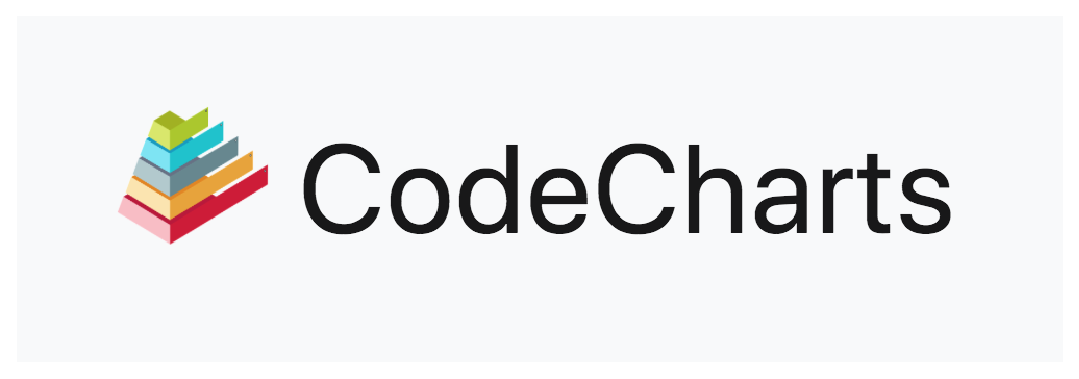
\includegraphics[width=0.5\textwidth]{images/logo_plataforma.eps}
\label{fig:9}
\end{center}
\end{figure}

En las siguientes secciones se describen en detalle la arquitectura y el diseño de la aplicación.

%++++++++++++++++++++++++++++++++++++++++++++++++++++++++++++++++++++++++++++++

\section{Arquitectura de la aplicación}
\label{4:sec:1}

\subsection{CodeCharts}
\label{1:sec:1}

CodeCharts fue desarrollado en Ruby on Rails, como se menciona en el punto 3.3.1, siguiendo la estructura en este tipo de proyectos ``MVC'' (Modelo, Vista, Controlador), así como el resto de herramientas que se describen en dicho capítulo.

%++++++++++++++++++++++++++++++++++++++++++++++++++++++++++++++++++++++++++++++

\newpage
\subsection{Base de datos}
\label{1:sec:2}

Desde un principio se usó una base de datos relacional, que nos proporcionaba Rails a través de SQLite y ActiveRecord.

\begin{figure}[!th]
\begin{center}
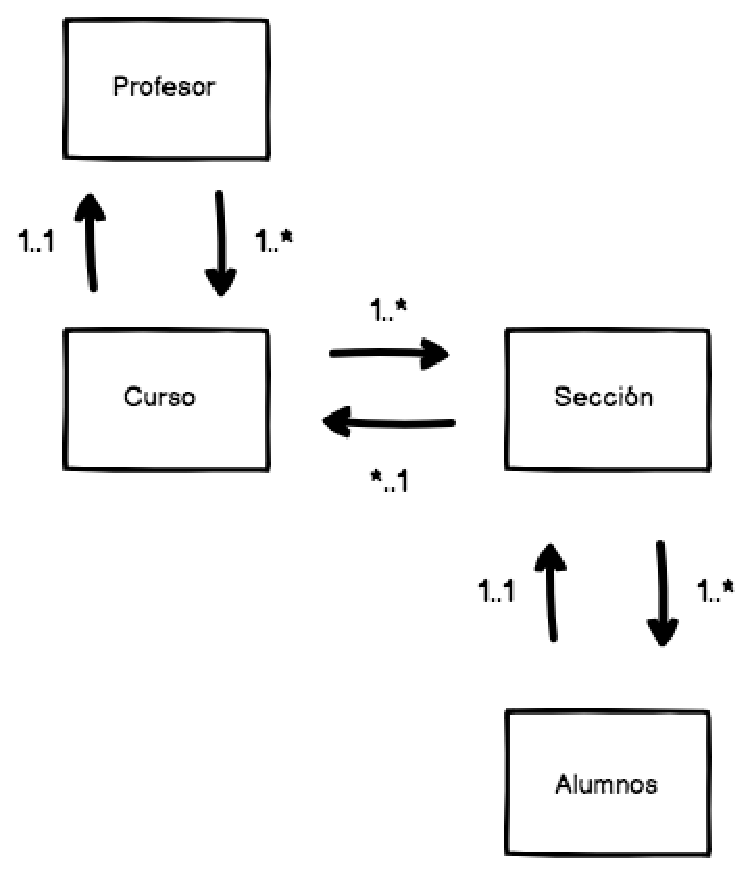
\includegraphics[width=0.4\textwidth]{images/base_de_datos.eps}
\caption{Esquema de la Base de Datos}
\label{fig:10}
\end{center}
\end{figure}

Como se muestra en la figura~\ref{fig:10}, la estructura de la base de datos se divide en cuatro tablas:

\begin{itemize}
    \item Profesor: donde se almacena toda la información referente a los profesores que se registren en la plataforma.
    \item Curso: creados por el profesorado, se guarda la información detallada del curso (título, descripción, etc.).
    \item Sección: se podría definir como el lugar de realización del curso, como por ejemplo ``Arona'', que tiene registrados a los alumnos con sus resultados en el mismo.
    \item Alumno: tabla en la que se almacenan los datos, así como los resultados, de los estudiantes que realizan los cursos o talleres de pensamiento computacional.
\end{itemize}

%++++++++++++++++++++++++++++++++++++++++++++++++++++++++++++++++++++++++++++++

\subsection{Gemas utilizadas}
\label{1:sec:3}

Una de las funcionalidades y características que tiene Ruby, el lenguaje usado para desarrollar el proyecto, es la incorporación de gemas, al igual que ocurre con el entorno NodeJS y sus paquetes ``npm''.

CodeCharts posee algunas relevantes como:

\begin{itemize}
    \item \textbf{Rails}, la gema que incluye Ruby on Rails por defecto para la utilización del framework.
    \item \textbf{SQLite}~\cite{SQLite}, para el manejo de las bases de datos, así como ActiveRecord.
    \item \textbf{Devise}~\cite{Devise}, que ofrece una solución flexible para la autenticación de los usuarios en la aplicación.
    \item \textbf{Bootstrap}~\cite{BootstrapGem}, gema que permite el diseño del front-end de la plataforma con Bootstrap.
    \item \textbf{Will-paginate}~\cite{Paginate}, de manera que si hay una gran cantidad de usuarios dentro de una sección, permita agruparlos en páginas.
    \item \textbf{Wicked-pdf}~\cite{WickedPDF}, con lo que el profesor puede descargar en formato .PDF los resultados de los alumnos.
    \item \textbf{Chartkick}, herramienta que muestra en forma gráfica los resultados obtenidos en los test de los estudiantes.
    \item \textbf{Jquery-rails}~\cite{JqueryRails}, que incluye Jquery en la aplicación. 
\end{itemize}

%++++++++++++++++++++++++++++++++++++++++++++++++++++++++++++++++++++++++++++++

\section{Diseño de la aplicación}
\label{1:sec:2}

\subsection{Página de inicio}
\label{1:sec:1}

La primera vez que se accede a la aplicación, el profesor, que será el usuario a registrarse en la plataforma, verá una descripción de en qué consiste la aplicación y lo que ofrece al profesorado en los cursos impartidos (véase la figura~\ref{fig:11}).

\begin{figure}[!th]
\begin{center}
\includegraphics[width=0.4\textwidth]{images/captura_inicio.eps}
\caption{Landing Page de CodeCharts}
\label{fig:11}
\end{center}
\end{figure}

Dentro de está página, el profesor se podrá registrar por primera vez, o por el contrario, si ya dispone de una cuenta creada previamente, puede entrar con la misma.

%++++++++++++++++++++++++++++++++++++++++++++++++++++++++++++++++++++++++++++++

\subsection{Registro/Inicio de sesión}
\label{1:sec:2}

En esta sección se describe el entorno del profesor que puede tanto crearse una cuenta, como iniciar sesión con una ya creada, si ya se ha registrado previamente. 

\begin{figure}[!th]%
    \centering
    \subfloat{{\includegraphics[width=5cm]{images/registro.eps} }}%
    \qquad
    \subfloat{{\includegraphics[width=5cm]{images/inicio_sesion.eps} }}%
    \caption{Registro e inicio de sesión}%
    \label{fig:12}%
\end{figure}

La figura~\ref{fig:12} muestra el formulario de \textit{creación de usuario} para la plataforma, el cual es muy sencillo, dado que consta de los datos básicos que se solicitan en la gran mayoría de páginas, como su nombre y apellidos, su correo electrónico y una contraseña.

%++++++++++++++++++++++++++++++++++++++++++++++++++++++++++++++++++++++++++++++

\subsection{Cursos creados}
\label{1:sec:3}

Una vez que el profesor ha accedido a la plataforma por primera vez, se mostrará una página como la que se observa en la figura~\ref{fig:13}. En ella se puede observar que se le informa al usuario que no tiene creado ningún curso/taller para sus alumnos, 
con lo que puede crearlos a través del botón de la parte superior izquierda.

\newpage
\begin{figure}[!th]
\begin{center}
\includegraphics[width=0.6\textwidth]{images/captura_cursos.eps}
\caption{Página de los cursos del profesor}
\label{fig:13}
\end{center}
\end{figure}

Los cursos creados se irán mostrando al profesor en forma de cuadrícula, de manera que el tutor sepa los cursos que tiene creados, con su información asociada (título, descripción y fecha de creación). Esto se muestra en la figura~\ref{fig:14}.

\begin{figure}[!th]
\begin{center}
\includegraphics[width=0.6\textwidth]{images/cursos_creados.eps}
\caption{Cursos creados por el profesor}
\label{fig:14}
\end{center}
\end{figure}

%++++++++++++++++++++++++++++++++++++++++++++++++++++++++++++++++++++++++++++++

\subsection{Perfil del profesor}
\label{1:sec:4}

Al profesor que haya iniciado sesión en ese momento, se le permitirá la opción de editar su perfil, a la vez que borrar su cuenta en caso de que ya no vaya a usar su cuenta en la plataforma.
Para que cualquier cambio, como se informa en el formulario, es necesaria la contraseña actual (Figura~\ref{fig:15}).

\begin{figure}[!th]
\begin{center}
\includegraphics[width=0.4\textwidth]{images/editar_perfil.eps}
\caption{Formulario para editar perfil del profesor}
\label{fig:15}
\end{center}
\end{figure}

%++++++++++++++++++++++++++++++++++++++++++++++++++++++++++++++++++++++++++++++

\newpage
\subsection{Detalles del curso}
\label{1:sec:5}

En el momento que el docente cree el curso o taller, podrá acceder para observar los detalles del mismo, así como crear secciones dentro de la actividad (Figura~\ref{fig:16}).

\begin{figure}[!th]
\begin{center}
\includegraphics[width=0.6\textwidth]{images/detalles_curso.eps}
\caption{Página con detalles del curso}
\label{fig:16}
\end{center}
\end{figure}

Al igual que con la página de las actividades, se le comunica al profesor que para observar las estadísticas de ese curso, tiene que añadir el lugar (Sección) donde se celebró el taller.
Uno de los detalles a destacar en el curso sería el de ``Valor de referencia", que se podría definir como un número representativo que indica el nivel que tienen los alumnos de media que realizan
esa actividad.

\begin{figure}[!th]
\begin{center}
\includegraphics[width=0.6\textwidth]{images/curso_secciones.eps}
\caption{Secciones creadas dentro del curso}
\label{fig:17}
\end{center}
\end{figure}

En la figura~\ref{fig:17} se puede observar un curso creado de ejemplo, junto con las secciones donde se realizó el curso. Tiene tanto la posibilidad de administrar a los alumnos, como se muestra en el botón derecha, al igual que eliminarlo.

%++++++++++++++++++++++++++++++++++++++++++++++++++++++++++++++++++++++++++++++

\newpage
\subsection{Detalles de la sección}
\label{1:sec:6}

El objetivo final de la plataforma es que el profesor, cuando inserte los resultados de los alumnos obtenidos de la plataforma Code.org, observe con gráficos las calificaciones de cada uno.

\begin{figure}[!th]
\begin{center}
\includegraphics[width=0.7\textwidth]{images/lista_sin_alumnos.eps}
\label{fig:18}
\end{center}
\end{figure}

\begin{figure}[!th]
\begin{center}
\includegraphics[width=0.3\textwidth]{images/insertar_alumnos.eps}
\caption{Introducción de alumnos de manera manual}
\label{fig:19}
\end{center}
\end{figure}

\newpage
Se pueden registrar alumnos en la plataforma tanto de manera manual de uno en uno (véase la figura~\ref{fig:19}), como a través de un fichero .JSON (véase la figura~\ref{fig:20}) con la información requerida, entre la que se encuentra el nombre, apellidos, edad, etc. Entre los datos más relevantes,
los niveles completados en ese reto, así como las líneas de código utilizadas en total.

\begin{figure}[!th]
\begin{center}
\includegraphics[width=0.7\textwidth]{images/subir_fichero.eps}
\caption{Subir ficheros de alumnos}
\label{fig:20}
\end{center}
\end{figure}

Al finalizar los retos por parte de los alumnos, el profesor obtendrá una tabla con toda la información de cada uno paginados, de manera que la tabla no se vuelva muy extensa al matricular a muchos alumnos, como se muestra en la figura~\ref{fig:21}.

\begin{figure}[!th]
\begin{center}
\includegraphics[width=0.7\textwidth]{images/tabla_alumnos.eps}
\caption{Tabla de ejemplo de alumnos matriculados}
\label{fig:21}
\end{center}
\end{figure}

\newpage
Por otro lado, en el apartado de estadísticas, se mostrarán gráficos desarrollados con la intención de ver en qué nivel se fomenta el aprendizaje en los alumnos.

\begin{figure}[!th]
\begin{center}
\includegraphics[width=0.7\textwidth]{images/estadisticas_seccion.eps}
\caption{Apartado de estadísticas}
\label{fig:22}
\end{center}
\end{figure}

En la figura~\ref{fig:22} se pueden observar algunos de los resultados obtenidos en forma de gráficos por los alumnos en ese curso.
   
  %%%%%%%%%%%%%%%%%%%%%%%%%%%%%%%%%%%%%%%%%%%%%%%%%%%%%%%%%%%%%%%%%%%%%%%%%%%%%%%
  \newpage{\pagestyle{empty}}
  \thispagestyle{empty}
   
  \chapter{Conclusiones y líneas futuras}
  \label{chapter:Conclusiones}
   
  %%%%%%%%%%%%%%%%%%%%%%%%%%%%%%%%%%%%%%%%%%%%%%%%%%%%%%%%%%%%%%%%%%%%%%%%%%%%%
% Chapter 5: Verificación y pruebas
%%%%%%%%%%%%%%%%%%%%%%%%%%%%%%%%%%%%%%%%%%%%%%%%%%%%%%%%%%%%%%%%%%%%%%%%%%%%%%%

En este capítulo se describen algunas de las pruebas realizadas para probar ciertos aspectos de la plataforma durante el desarrollo del proyecto, así como los problemas que se presentaron a la hora de realizar la aplicación.

%++++++++++++++++++++++++++++++++++++++++++++++++++++++++++++++++++++++++++++++

\section{Problemas encontrados}
\label{5:sec:1}

Durante el proceso de desarrollo del Trabajo Fin de Grado, surgieron diversos problemas para llevar a cabo la integración de la herramienta para la representación gráfica de los resultados de los alumnos.

En primer lugar, se decidió que la plataforma ``Code.org'' era la más completa al disponer de retos suficientes para los profesores, de manera que fomenten el aprendizaje del pensamiento computacional. A través de su repositorio en Github, donde
se aloja toda la página, se realizó un estudio para comprobar de qué manera estaba estructurada la página y posteriormente se procedió a intentar realizar la contribución.

Al comprobar que su estructura se actualizaba constantemente en el repositorio y era imposible integrar la herramienta, se diseñó un servicio web externo. Este servicio, como se explica en puntos anteriores, 
funciona de manera similar a Code.org, con la particularidad de que se añade la información de los alumnos una vez hayan finalizado el curso en el lugar (sección) que se esté realizando.

%++++++++++++++++++++++++++++++++++++++++++++++++++++++++++++++++++++++++++++++

\section{Testeo de la aplicación}
\label{5:sec:2}

Como se describió en el apartado de ``Tecnología utilizada'', las pruebas se realizaron con RSpec. Las pruebas se ejecutaron sobre alguno de los modelos de la aplicación:

\begin{itemize}
    \item \textbf{Curso}: se validan que los atributos que se le pasan al curso de ejemplo son correctos. A su vez, si un curso tiene una o más secciones, así como insertar cursos en la aplicación.
    \begin{figure}[!th]
    \begin{center}
    \includegraphics[width=0.6\textwidth]{images/pruebas_curso.eps}
    \caption{Pruebas realizadas al modelo de cursos}
    \label{fig:23}
    \end{center}
    \end{figure}
    
    \item \textbf{Sección}: para este modelo se comprueba que, tanto las secciones como los usuarios en las mismas, se crean correctamente, de igual manera que se pueden eliminar los usuarios.
    \begin{figure}[!th]
    \begin{center}
    \includegraphics[width=0.6\textwidth]{images/pruebas_seccion.eps}
    \caption{Pruebas realizadas al modelo de las secciones}
    \label{fig:24}
    \end{center}
    \end{figure}
    \item \textbf{Usuarios}: al igual que con la sección, se valida que se pueden introducir manualmente con éxito.
\end{itemize}

\newpage
Por último, como se observa en la imagen, una vez que se ejecuta el comando ``rspec -fd'', nos muestra el título de cada una de las pruebas y en la parte inferior la cantidad de pruebas que se realizaron
y, en caso de errores, nos lo indicaría. En este caso, todas las pruebas pasan correctamente.

\begin{figure}[!th]
\begin{center}
\includegraphics[width=0.5\textwidth]{images/resultado_pruebas.eps}
\caption{Pruebas realizadas al modelo de las secciones}
\label{fig:25}
\end{center}
\end{figure}
   
  %%%%%%%%%%%%%%%%%%%%%%%%%%%%%%%%%%%%%%%%%%%%%%%%%%%%%%%%%%%%%%%%%%%%%%%%%%%%%%%
  \newpage{\pagestyle{empty}}
  \thispagestyle{empty}
   
  \chapter{Summary and Conclusions }
  \label{chapter:ingles}
   
  %%%%%%%%%%%%%%%%%%%%%%%%%%%%%%%%%%%%%%%%%%%%%%%%%%%%%%%%%%%%%%%%%%%%%%%%%%%%%
% Chapter 6: Summary and Conlusions
%%%%%%%%%%%%%%%%%%%%%%%%%%%%%%%%%%%%%%%%%%%%%%%%%%%%%%%%%%%%%%%%%%%%%%%%%%%%%%%

%---------------------------------------------------------------------------------

La plataforma desarrollada, llamada CodeCharts, pretende facilitar al profesorado la visualización del progreso de sus alumnos, de manera que una vez que los estudiantes hayan realizado los retos, puedan comprobar en qué medida los cursos
o talleres están ayudando en el fomento del pensamiento computacional a la hora de afrontar las actividades.

Una de las peculiaridades de esta plataforma es que está pensada para que solo la use el personal de la docencia, por ello se ha desarrollado para su uso de la manera más sencilla y cómoda. En el momento que el profesor disponga de todos los datos de los alumnos,
sólo debe proceder a introducirlos en la web, y ya podrá disfrutar de la funcionalidad que lo define, las estadísticas.





   
  %%%%%%%%%%%%%%%%%%%%%%%%%%%%%%%%%%%%%%%%%%%%%%%%%%%%%%%%%%%%%%%%%%%%%%%%%%%%%%%
  \newpage{\pagestyle{empty}}
  \thispagestyle{empty}
   
  \chapter{Presupuesto}
  \label{chapter:Presupuesto}
   
  %%%%%%%%%%%%%%%%%%%%%%%%%%%%%%%%%%%%%%%%%%%%%%%%%%%%%%%%%%%%%%%%%%%%%%%%%%%%%
% Chapter 7: Presupuesto
%%%%%%%%%%%%%%%%%%%%%%%%%%%%%%%%%%%%%%%%%%%%%%%%%%%%%%%%%%%%%%%%%%%%%%%%%%%%%%%

%++++++++++++++++++++++++++++++++++++++++++++++++++++++++++++++++++++++++++++++

Este capítulo es obligatorio.
Toda memoria de Trabajo de Fin de Grado debe incluir un presupuesto.

%---------------------------------------------------------------------------------
\section{Sección Uno}
\label{7:sec:1}


%--------------------------------------------------------------------------
\begin{table}[!ht]
\begin{center}
\begin{tabular}{|p{60mm}|p{20mm}|p{40mm}|p{25mm}|} \hline 
\textbf{Recurso} & \textbf{Horas} & \textbf{Precio unidad} & \textbf{Total}\\ \hline
Estudio Pensamiento Computacional & 50 & 12\euro & 600\euro \\ \hline

Tutorial Ruby on Rails & 10 & 12\euro & 120\euro \\ \hline

Desarrollo de plataforma & 10 & 10\euro & 100\euro \\ \hline

Front-End & 50 & 12\euro & 600\euro \\ \hline

Back-End & 60 & 12\euro & 720\euro \\ \hline

Total & 170 & - &  \\ \hline

\end{tabular}
\end{center}
\caption{Tabla resumen del presupuesto}
\label{table:resOthers}
\end{table}




   
  %%%%%%%%%%%%%%%%%%%%%%%%%%%%%%%%%%%%%%%%%%%%%%%%%%%%%%%%%%%%%%%%%%%%%%%%%%%%%%%
   
  %%%%%%%%%%%%%%%%%%%%%%%%%%%%%%%%%%%%%%%%%%%%%%%%%%%%%%%%%%%%%%%%%%%%%%%%%%%%%%%
  \newpage{\pagestyle{empty}}
  \thispagestyle{empty}
  \begin{appendix}
   
  \chapter{Título del Apéndice 1}
  \label{appendix:1}
  \section{Algoritmo XXX}
\label{Apendice1:XXX}

\begin{center}
\begin{footnotesize}
\begin{verbatim}

***********************************************************************************
*
* Fichero .h
*
***********************************************************************************
*
* AUTORES
*   
*
* FECHA
*   
*
* DESCRIPCION
*   
*
************************************************************************************/

\end{verbatim}
\end{footnotesize}
\end{center}

\section{Algoritmo YYY}
\label{Apendice1:YYY}

\begin{center}
\begin{footnotesize}
\begin{verbatim}


/***********************************************************************************
 *
 * Fichero .h
 *
 ***********************************************************************************
 *
 * AUTORES
 *
 * FECHA
 *
 * DESCRIPCION
 *
 *
 ************************************************************************************/

\end{verbatim}
\end{footnotesize}
\end{center}

   
  \chapter{Título del Apéndice 2}
  \label{appendix:2}
  \section{Otro apéndice: Sección 1}
\label{Apendice2:label}

\begin{center}
\begin{footnotesize}

\begin{verbatim}
Texto
\end{verbatim}

\end{footnotesize}
\end{center}

\section{Otro apéndice: Sección 2}
\label{Apendice2:label2}

\begin{center}
\begin{footnotesize}

\begin{verbatim}
Texto
\end{verbatim}


\end{footnotesize}
\end{center}

   
  \end{appendix}
   
  %%%%%%%%%%%%%%%%%%%%%%%%%%%%%%%%%%%%%%%%%%%%%%%%%%%%%%%%%%%%%%%%%%%%%%%%%%%%%%%
  \addcontentsline{toc}{chapter}{Bibliografía}
  \bibliographystyle{plain}
   
  \bibliography{memtfg}
  %\nocite{*}
   
  %%%%%%%%%%%%%%%%%%%%%%%%%%%%%%%%%%%%%%%%%%%%%%%%%%%%%%%%%%%%%%%%%%%%%%%%%%%%%%%
   
  \end{document}